% Bachelor defense deck — DTU-styled Beamer (xelatex), MLOps-forward.
% Structure (sandwich): present the system -> LIVE DEMO (middle) -> results & conclusions.
% Build:  latexmk -xelatex defense.tex   (run from Report/Presentation/)
\documentclass[aspectratio=169,10pt]{beamer}

\usepackage{fontspec}
\setsansfont{Liberation Sans}
\setmainfont{Liberation Sans}
\usepackage{booktabs}
\usepackage{colortbl}
\usepackage{amsmath}
\usepackage{amssymb}   % \blacktriangleright for the demo slide

\graphicspath{%
  {../figures/system_implementation/}%
  {../figures/methods_models/}%
  {../figures/results_models/}%
  {../Pictures/Logos/}%
}

% ---- DTU colours ----
\definecolor{dtured}{rgb}{0.6,0,0}
\definecolor{dtugrey}{rgb}{0.85,0.85,0.85}
\definecolor{dtudark}{rgb}{0.18,0.18,0.18}

% ---- minimal DTU-ish theme ----
\setbeamercolor{structure}{fg=dtured}
\setbeamercolor{frametitle}{fg=dtured}
\setbeamercolor{title}{fg=white}
\setbeamercolor{normal text}{fg=dtudark}
\setbeamercolor{itemize item}{fg=dtured}
\setbeamercolor{itemize subitem}{fg=dtured}
\setbeamercolor{block title}{bg=dtured,fg=white}
\setbeamercolor{block body}{bg=dtugrey!30}
\setbeamerfont{frametitle}{series=\bfseries}
\setbeamertemplate{navigation symbols}{}
\setbeamertemplate{itemize items}[circle]

\setbeamertemplate{frametitle}{%
  \vskip0.6em\hbox{\insertframetitle}%
  \vskip2pt{\color{dtured}\rule{\textwidth}{1.2pt}}%
}
\setbeamertemplate{footline}{%
  \hbox{\begin{beamercolorbox}[wd=\paperwidth,ht=2.4ex,dp=1ex,leftskip=1.2em,rightskip=1.2em]{}%
    {\color{dtured}\scriptsize An MLOps platform for day-ahead EPF}\hfill
    {\color{dtured}\scriptsize Viet Hoang Nguyen \;|\; DTU Compute \;|\; \insertframenumber}%
  \end{beamercolorbox}}%
}

\title{Designing an Algorithmic System for Energy Market Forecasting}
\author{Viet Hoang Nguyen \,(s234859)}
\institute{DTU Compute \\ Supervisor: Finn Årup Nielsen}
\date{June 2026}

\begin{document}

% =====================================================
% PART 1 — THE PROBLEM & THE PLATFORM  (~6-7 min)
% =====================================================

% ----- 1. TITLE -----
{%
\setbeamercolor{background canvas}{bg=dtured}
\begin{frame}[plain]
  \color{white}
  \vskip1.2em
  
\includegraphics[height=1.1cm]{white_rgb}
  \vfill
  {\Large\bfseries Designing an Algorithmic System for\\[2pt]
   Energy Market Forecasting}\\[4pt]
  {\normalsize Benchmark EPF models inside an \textbf{MLOps platform}}\\[1.4em]
  {\small Bachelor's thesis defense}\\[0.3em]
  {\small Viet Hoang Nguyen \,(s234859)}\\[0.2em]
  {\footnotesize DTU Compute \quad$\cdot$\quad Supervisor: Finn Årup Nielsen \quad$\cdot$\quad June 2026}
  \vfill
\end{frame}
}

% ----- 2. MOTIVATION + GAP -----
\begin{frame}{Forecasting models must be operated, not just built}
  \begin{columns}[T]
    \begin{column}{0.5\textwidth}
      \textbf{EPF research}
      \begin{itemize}\small
        \item Produces accurate benchmark models.
        \item Evaluates them \textbf{offline, once}.
      \end{itemize}
    \end{column}
    \begin{column}{0.5\textwidth}
      \textbf{Production reality}
      \begin{itemize}\small
        \item A served model must be \textbf{retrained, monitored, reproduced, audited}.
        \item That operational layer is what \textbf{MLOps} addresses --- and EPF research
          leaves out.
      \end{itemize}
    \end{column}
  \end{columns}
  \vfill
  \begin{block}{This thesis}
    Build a production \textbf{MLOps platform} that operates benchmark EPF models, and
    \textbf{evaluate the platform itself}. The two fields rarely meet (only Subramanya et
    al.).
  \end{block}
\end{frame}

% ----- 3. AIM + RQs -----
\begin{frame}{Aim and research questions}
  A platform that ingests ENTSO-E data, recalibrates and forecasts \textbf{daily} for DK1
  and DE, \textbf{monitors} quality and drift, and keeps \textbf{full provenance}.
  \vfill
  \begin{enumerate}
    \item[\textbf{RQ1}] \textbf{Forecasting} --- how do replicated LEAR, DNN and
      Transformer compare? \emph{(the workload the platform serves)}
    \item[\textbf{RQ2}] \textbf{Engineering} --- what trade-offs emerge when
      productionising these models?
    \item[\textbf{RQ3}] \textbf{Maturity} --- which of Zarour et al.'s nine MLOps practices
      does the platform realise, and where does a single-host MVP reach its limit?
  \end{enumerate}
\end{frame}

% ----- 4. THE PLATFORM (high-level system) -----
\begin{frame}{The platform \hfill\small(\S4.2)}
  \begin{columns}[c]
    \begin{column}{0.60\textwidth}
      \centering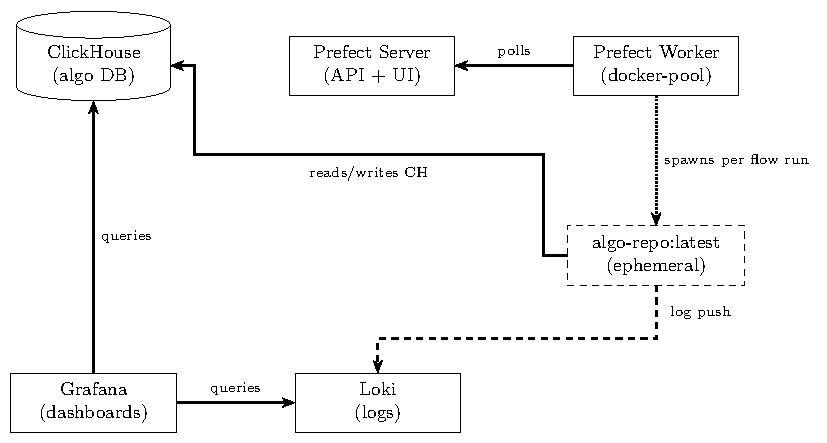
\includegraphics[width=\linewidth]{f1-architecture}
    \end{column}
    \begin{column}{0.40\textwidth}
      \begin{itemize}
        \item One Docker host, \textbf{six services}: ClickHouse, Prefect
          (server + worker), Prometheus, Grafana, Loki.
        \item Flow runs spawn ephemeral \texttt{algo-repo} containers.
        \item Daily loop (UTC): \textbf{06:00} forecast, \textbf{18:00} reconcile,
          \textbf{19:00} drift.
        \item Serves three benchmark EPF models on DK1 and DE.
      \end{itemize}
    \end{column}
  \end{columns}
\end{frame}

% ----- 5. DATA PLANE (high-level system) -----
\begin{frame}{One data path, end to end \hfill\small(\S4.2)}
  \begin{columns}[c]
    \begin{column}{0.58\textwidth}
      \centering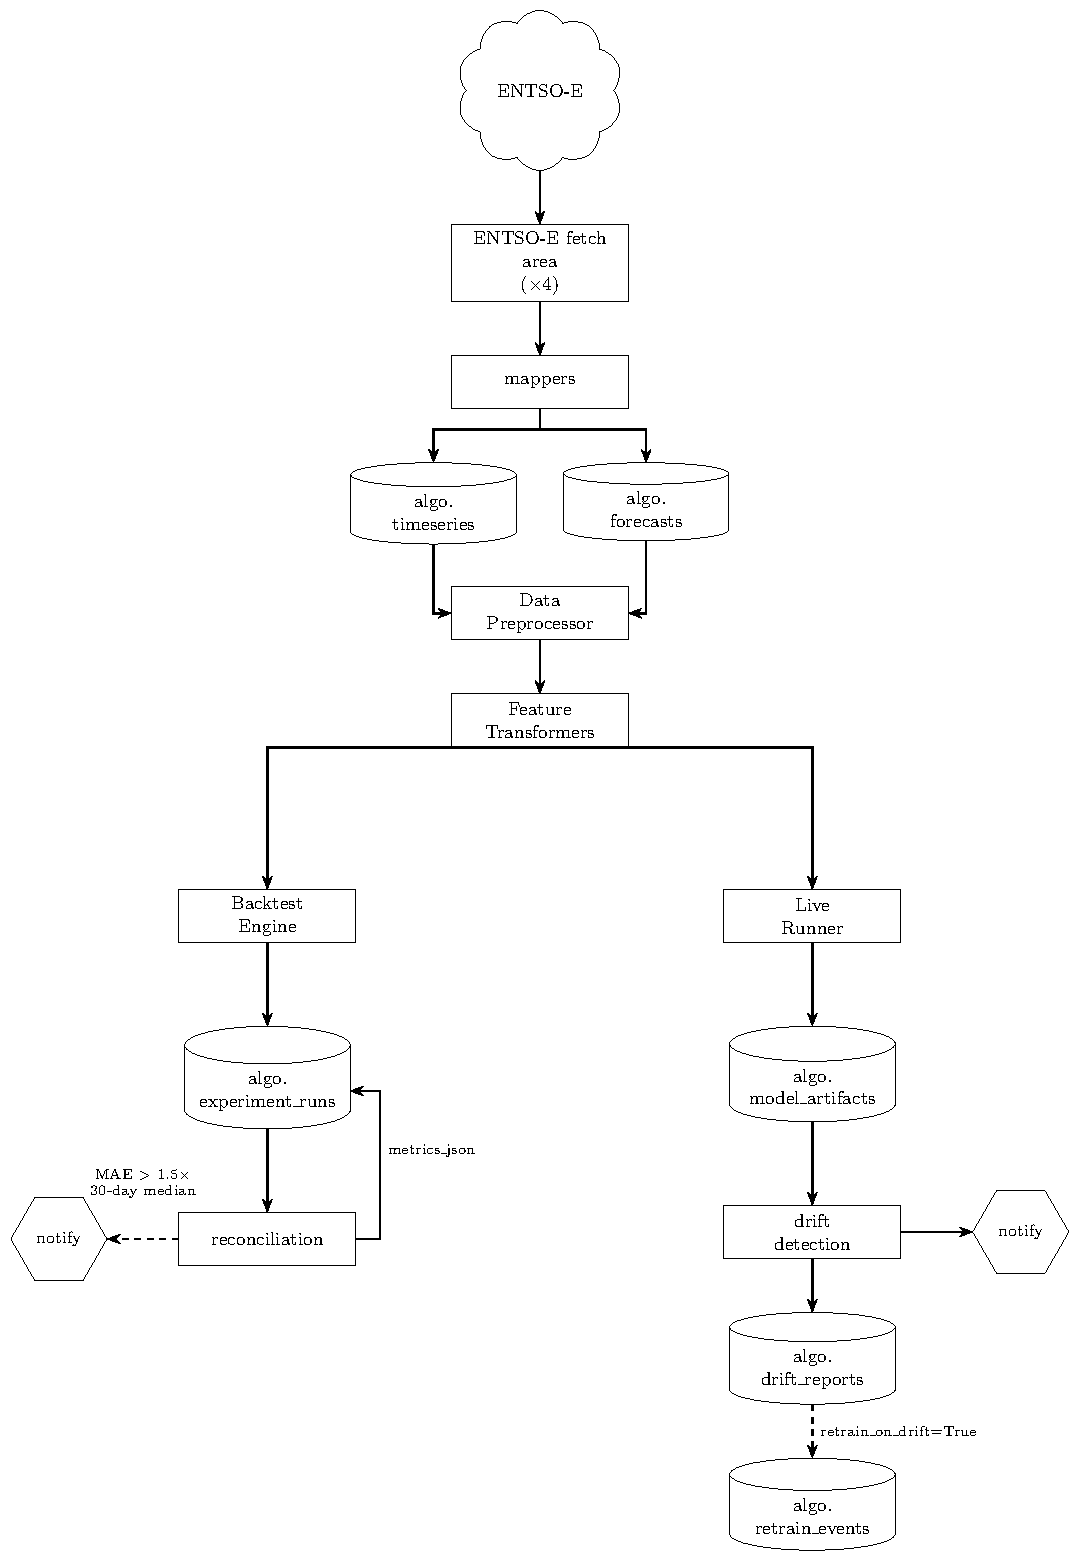
\includegraphics[width=\linewidth]{f2-data-plane}
    \end{column}
    \begin{column}{0.42\textwidth}
      \begin{itemize}\small
        \item ENTSO-E $\to$ XML mappers $\to$ ClickHouse
          (\texttt{timeseries}, \texttt{forecasts}; \texttt{ReplacingMergeTree}).
        \item Preprocessor $\to$ backtest / live runner $\to$ predictions + artefacts.
        \item Reconciliation back-fills actuals; drift compares distributions and can
          raise alerts or retraining.
      \end{itemize}
    \end{column}
  \end{columns}
\end{frame}

% ----- 6. NINE PRACTICES -----
\begin{frame}{Built around nine MLOps practices \hfill\small(Zarour et al.)}
  \footnotesize
  \begin{columns}[T]
    \begin{column}{0.5\textwidth}
      \begin{tabular}{ll}
        \textbf{P1} CI/CD            & GitHub Actions \\[2pt]
        \textbf{P2} Orchestration    & Prefect flows \\[2pt]
        \textbf{P3} Reproducibility  & GIT\_SHA + Compose \\[2pt]
        \textbf{P4} Versioning       & Git + migrations \\[2pt]
        \textbf{P5} Collaboration    & PRs + versioned docs \\
      \end{tabular}
    \end{column}
    \begin{column}{0.5\textwidth}
      \begin{tabular}{ll}
        \textbf{P6} Train \& evaluate& daily forecast + reconcile \\[2pt]
        \textbf{P7} Metadata         & ClickHouse + W\&B \\[2pt]
        \textbf{P8} Monitoring       & Grafana / Loki / Prometheus \\[2pt]
        \textbf{P9} Feedback loops   & drift $\to$ retrain (opt-in) \\
      \end{tabular}
    \end{column}
  \end{columns}
  \vfill
  \centering These structure the system chapter --- and I will show seven of them running
  \textbf{live, next}.
\end{frame}

% =====================================================
% PART 2 — LIVE DEMO  (~7.5 min, the middle)
% =====================================================
{%
\setbeamercolor{background canvas}{bg=dtured}
\begin{frame}[plain]
  \color{white}\centering
  \vfill
  {\Huge\bfseries $\blacktriangleright$\; LIVE DEMO}\\[10pt]
  {\large Adding a new market (DK2), end to end}\\[14pt]
  {\normalsize CI/CD \quad$\cdot$\quad Prefect \quad$\cdot$\quad Grafana \quad$\cdot$\quad W\&B}\\[16pt]
  {\small\itshape ``A contributor adds DK2 and ships it to a live, monitored forecast.''}
  \vfill
  {\footnotesize seven of the nine practices --- running}
  \vfill
\end{frame}
}

% =====================================================
% PART 3 — RESULTS, EVALUATION & CONCLUSIONS  (~6.5 min)
% =====================================================

% ----- 8. THE WORKLOAD -----
\begin{frame}{The workload: three benchmark models \hfill\small(\S3.1, 3.3)}
  \begin{itemize}\small
    \item \textbf{LEAR} --- one Lasso per delivery hour (Lago et al.).
    \item \textbf{DNN} --- MLP mapping the feature vector to all 24 hours at once (MIMO).
    \item \textbf{Transformer} --- encoder-only, two input branches (Llorente \& Portela).
  \end{itemize}
  \vfill
  \begin{block}{Replication framing}
    Faithful \textbf{in specification}, on current DK1 + DE data. Because the price regime
    differs from the 2016--2018 source-paper era, the comparison is read in \textbf{relative}
    terms (rMAE and rankings), with paired \textbf{Giacomini--White} significance tests.
  \end{block}
\end{frame}

% ----- 9. RQ1 ACCURACY -----
\begin{frame}{RQ1 --- accuracy and significance \hfill\small(\S5.1--5.2)}
  \begin{columns}[T]
    \begin{column}{0.5\textwidth}
      \footnotesize
      \textbf{rMAE} (common days, $\downarrow$ better)\\[2pt]
      \begin{tabular}{lcc}
        \toprule
         & DK1 & DE \\
        \midrule
        LEAR        & \textbf{0.469} & \textbf{0.376} \\
        DNN         & 0.482 & 0.388 \\
        Transformer & 0.543 & 0.420 \\
        Naive (weekly) & 1.000 & 1.000 \\
        \bottomrule
      \end{tabular}
      \vskip0.7em
      \begin{itemize}\footnotesize
        \item LEAR $\approx$ DNN, \textbf{indistinguishable} ($p=0.16/0.19$).
        \item Both \textbf{beat} the Transformer ($p\le0.013$); all beat the naive.
      \end{itemize}
    \end{column}
    \begin{column}{0.48\textwidth}
      \centering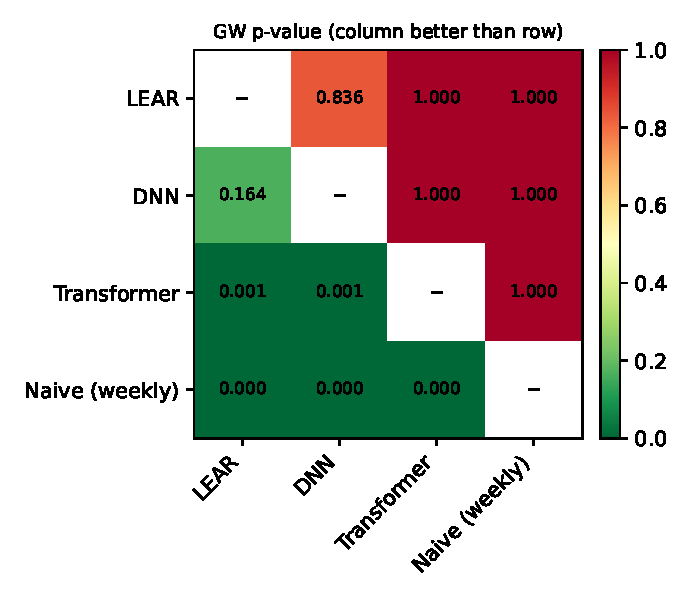
\includegraphics[width=0.9\linewidth]{gw_heatmap_dk1}\\
      {\scriptsize Giacomini--White p-values, DK1.}
    \end{column}
  \end{columns}
\end{frame}

% ----- 10. RQ1 COST + PAPERS -----
\begin{frame}{RQ1 --- cost, and ranking vs the papers \hfill\small(\S5.3--5.4)}
  \begin{columns}[T]
    \begin{column}{0.46\textwidth}
      \footnotesize \textbf{Cost} (s / recalibration-day)
      \begin{tabular}{lcc}
        \toprule
         & DK1 & DE \\
        \midrule
        LEAR (CPU)   & 50.3 & 41.3 \\
        DNN (GPU)    & 0.9  & 1.6 \\
        Transf.(GPU) & 1.6  & 1.9 \\
        \bottomrule
      \end{tabular}
      \vskip0.4em
      The DNN gives \textbf{equal accuracy for far less compute}.
    \end{column}
    \begin{column}{0.54\textwidth}
      \begin{itemize}\footnotesize
        \item Our order LEAR $\ge$ DNN $\ge$ Transformer \textbf{inverts both papers}.
        \item LEAR--DNN inversion is only numerical (they are tied).
        \item Transformer's third place is genuine and significant.
        \item \textbf{Most consistent with} the deep models' reduced tuning budget
          (DNN 30 trials vs the paper's 1500), not weaker architectures --- a hypothesis,
          confirmatory run is future work.
      \end{itemize}
    \end{column}
  \end{columns}
\end{frame}

% ----- 11. RQ3 EVALUATION -----
\begin{frame}{RQ3 --- maturity and quantitative evaluation \hfill\small(\S6.1--6.4)}
  \begin{columns}[c]
    \begin{column}{0.5\textwidth}
      \footnotesize
      \begin{tabular}{llc}
        \toprule
        Practice & Status & Lvl \\
        \midrule
        P1 CI/CD            & Realised & 2 \\
        P2 Orchestration    & Realised & 2 \\
        P3 Reproducibility  & Realised & 2 \\
        P4 Versioning       & Realised & 2 \\
        P5 Collaboration    & Realised & 1 \\
        P6 Train \& evaluate& Realised & 1 \\
        P7 Metadata         & Realised & 1 \\
        P8 Monitoring       & Realised & 2 \\
        P9 Feedback loops   & \textbf{Minimal} & 1 \\
        \bottomrule
      \end{tabular}
    \end{column}
    \begin{column}{0.5\textwidth}
      \textbf{8 of 9 realised}; 1 minimal. Backed by numbers:
      \begin{itemize}\footnotesize
        \item \textbf{ML Test Score 2.5} (min of sections), bound by data testing.
        \item Provenance \textbf{66.7\%}, 100\% from the first CD run.
        \item A logged forecast re-ran to \textbf{$7\times10^{-6}$ EUR/MWh}.
      \end{itemize}
      \vskip0.3em
      \footnotesize DevOps practices transferred easily; ML-specific data testing is where
      the MVP is weakest.
    \end{column}
  \end{columns}
\end{frame}

% ----- 12. RQ2 -----
\begin{frame}{RQ2 --- engineering trade-offs \hfill\small(\S7.2)}
  \begin{itemize}
    \item Productionising the benchmark models \textbf{mostly aligned} the needs of a
      faithful replication and a single-host MVP --- both favour determinism and a single
      source of truth.
    \item \textbf{Full refit from scratch} each day: cheap, avoids warm-start error, makes
      drift-triggered retraining redundant.
    \item \textbf{One OLAP store} for data, predictions, metrics, artefacts $\Rightarrow$
      reconciliation is one query.
  \end{itemize}
  \vfill
  \begin{block}{A genuine tension I resolved}
    The Transformer's native \emph{train-once + renormalise} scheme vs the daily-refit
    pipeline. I chose production consistency and deviated from the paper.
  \end{block}
\end{frame}

% ----- 13. CONCLUSION -----
\begin{frame}{Conclusion and future work}
  \begin{block}{Contribution}
    A reproducible, monitored MLOps platform that operates three benchmark-faithful EPF
    models, with a quantified \textbf{maturity evaluation} and a significance-tested model
    comparison --- joining MLOps and EPF in one artifact.
  \end{block}
  \vskip0.3em
  \textbf{Result:} 8 of 9 practices realised; ML Test Score 2.5; reproducible to
  $7\times10^{-6}$ EUR/MWh. LEAR and the DNN tied at the top, Transformer weaker.
  \vskip0.5em
  \textbf{Future work:} probabilistic forecasting (CRPS); close the replication gap (full
  tuning + \texttt{epftoolbox} side-by-side); recalibrate drift and broaden coverage;
  controlled re-run of the stochastic models.
\end{frame}

% ----- 14. THANKS -----
\begin{frame}[plain]
  \vfill\centering
  {\color{dtured}\Large\bfseries Thank you --- questions?}\\[1em]
  {\footnotesize Backup slides follow: the nine practices in detail, system internals,
  and forecasting / statistics deep-dives.}
  \vfill
\end{frame}

% =====================================================
\appendix   % BACKUP — shown on demand during questions
% =====================================================

\begin{frame}[plain]
  \vfill\centering
  {\color{dtured}\Large\bfseries Backup slides}\\[2pt]
  {\color{dtured}\rule{0.4\textwidth}{1pt}}\\[6pt]
  {\footnotesize implementation detail $\cdot$ the nine practices $\cdot$ forecasting \& statistics}
  \vfill
\end{frame}

\begin{frame}{Backup --- tech stack and the alternatives rejected}
  \footnotesize
  \begin{tabular}{lll}
    \toprule
    Role & Chosen & Over \\
    \midrule
    Storage / OLAP        & ClickHouse (one store)       & a filesystem model store \\
    Orchestration         & Prefect                      & Airflow, Dagster \\
    Runtime               & Docker Compose               & Kubernetes \\
    Logs / metrics / dash & Loki + Prometheus + Grafana  & the ELK stack \\
    Experiment tracking   & Weights \& Biases            & MLflow (deferred) \\
    CI/CD                 & GitHub Actions               & Jenkins, CircleCI \\
    Secure deploy access  & Tailscale (ephemeral SSH)    & a public SSH port \\
    \bottomrule
  \end{tabular}
  \vfill
  \centering Every choice sized to a \textbf{single-host MVP}.
\end{frame}

\begin{frame}{Backup --- P1 Automated CI/CD \hfill\small(\S4.3.1)}
  \begin{columns}[c]
    \begin{column}{0.56\textwidth}
      \centering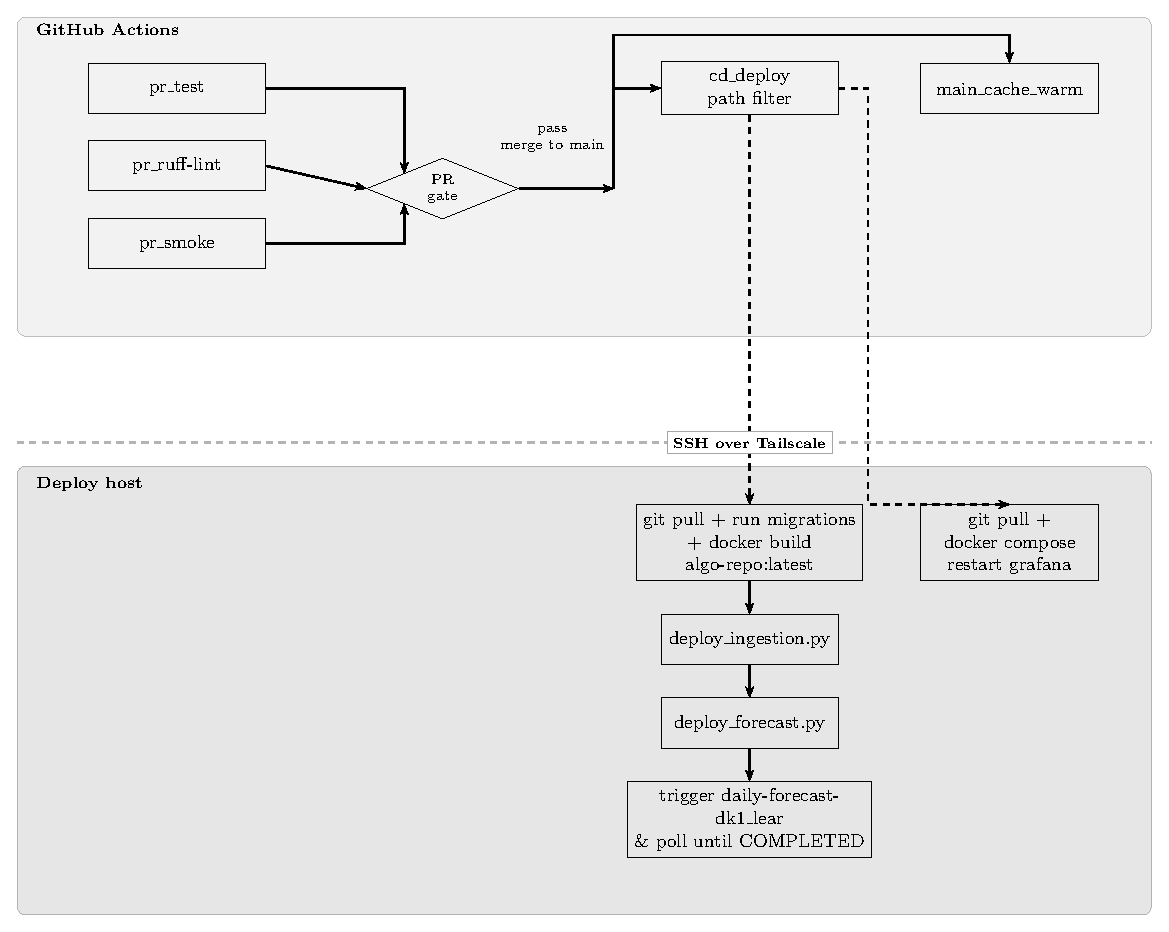
\includegraphics[width=\linewidth]{f3-cicd}
    \end{column}
    \begin{column}{0.44\textwidth}
      \begin{itemize}\small
        \item PR gates: \texttt{pr\_test}, \texttt{pr\_ruff-lint}, \texttt{pr\_smoke}.
        \item On merge: \texttt{cd\_deploy} over Tailscale, migrations, image rebuilt with
          the commit SHA, Prefect redeployed, smoke forecast.
      \end{itemize}
    \end{column}
  \end{columns}
\end{frame}

\begin{frame}{Backup --- P2 Orchestration \hfill\small(\S4.3.2)}
  \begin{itemize}\small
    \item Four Prefect flows on a Docker work pool: ingestion, forecast, reconciliation, drift.
    \item \textbf{16 deployments} from shared definitions, parameterised by area (one
      definition, one deployment per zone).
    \item One task per data type, sequential, \texttt{retries=2}; fetch/insert logic in a
      shared service with no Prefect dependency.
  \end{itemize}
\end{frame}

\begin{frame}{Backup --- P3 Reproducibility \hfill\small(\S4.3.3)}
  \begin{itemize}\small
    \item Whole stack in \texttt{docker-compose.yml}; rebuildable from the repo alone.
    \item \texttt{GIT\_SHA} baked into the image; local runs emit empty so a dirty tree
      never stamps a misleading SHA.
    \item Config-driven pipeline: calibration windows, \texttt{asinh} transform, enumerated
      seeds all pinned.
  \end{itemize}
\end{frame}

\begin{frame}{Backup --- P4 / P5 Versioning and collaboration \hfill\small(\S4.3.4--4.3.5)}
  \begin{itemize}\small
    \item Git tracks \texttt{configs/}, numbered SQL migrations, Grafana dashboards and
      alert rules.
    \item DVC evaluated and rejected --- ENTSO-E data is replayable; \texttt{ReplacingMergeTree}
      + \texttt{git\_sha} give provenance without a binary store.
    \item Every change via PR; conventions in versioned \texttt{REPO\_OVERVIEW} /
      \texttt{RUNBOOK} / \texttt{CONTRIBUTING}.
  \end{itemize}
\end{frame}

\begin{frame}{Backup --- P6 Continuous training and evaluation \hfill\small(\S4.3.6)}
  \begin{columns}[c]
    \begin{column}{0.54\textwidth}
      \centering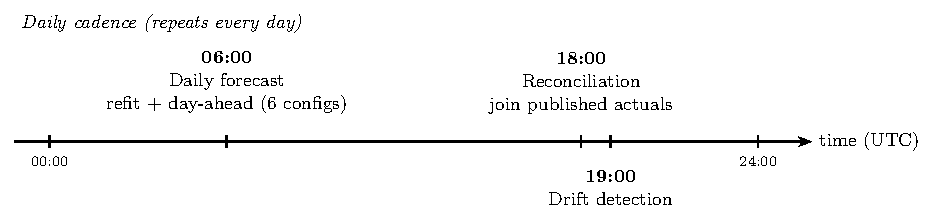
\includegraphics[width=\linewidth]{f5-daily-cadence}
    \end{column}
    \begin{column}{0.46\textwidth}
      \begin{itemize}\small
        \item Six \texttt{daily-forecast} deployments refit at 06:00; the DNN averages a
          4-seed ensemble.
        \item Each run refits from scratch on a rolling window.
        \item Reconciliation scores live forecasts next day with the same metrics as the
          backtest.
      \end{itemize}
    \end{column}
  \end{columns}
\end{frame}

\begin{frame}{Backup --- P7 Tracking ML metadata \hfill\small(\S4.3.7)}
  \begin{itemize}\small
    \item ClickHouse: \texttt{experiment\_runs} (git SHA, data window, duration),
      \texttt{experiment\_predictions}, \texttt{model\_artifacts}, \texttt{hyperparam\_trials}.
    \item W\&B research surface: \texttt{algo-research} (backtests, sweeps),
      \texttt{algo-prod} (reconciliation). \texttt{WANDB\_MODE=disabled} no-ops it in CI.
  \end{itemize}
\end{frame}

\begin{frame}{Backup --- P8 Continuous monitoring \hfill\small(\S4.3.8)}
  \begin{itemize}\small
    \item Three Grafana dashboards: Data Quality, System Health, Operational (Loki stream).
    \item Prometheus scrapes ClickHouse / Grafana / itself every 15 s.
    \item Five alert rules: staleness, drift-detected, reconciliation-missed,
      ClickHouse-down, accuracy-degradation ($>1.5\times$ 30-day median).
  \end{itemize}
\end{frame}

\begin{frame}{Backup --- P9 Feedback loops \hfill\small(\S4.3.9)}
  \begin{itemize}\small
    \item Drift (Evidently, 90-day vs 7-day) daily in-process; results in
      \texttt{drift\_reports}; detected events alert and can trigger an audited retrain.
    \item Trigger \textbf{off by design} --- the cheap daily refit keeps models fresh
      (cost-aware argument of Mahadevan \& Mathioudakis).
    \item The one \textbf{minimal} practice. Drift flagged 49/49 (over-powered) --- next
      step is seasonally-matched windows and testing residuals.
  \end{itemize}
\end{frame}

\begin{frame}{Backup --- features and the target transform \hfill\small(\S3.2)}
  \begin{columns}[c]
    \begin{column}{0.5\textwidth}
      \[ \underbrace{4n}_{\text{price lags}} + \underbrace{2\cdot 3n}_{\text{2 exog}\times\text{3 lags}} + \underbrace{7}_{\text{weekday}} = 247 \]
      \footnotesize ($n=24$). LEAR's Lasso shrinks most coefficients to zero; \texttt{asinh}
      tames spikes while staying defined for \textbf{negative} prices.
    \end{column}
    \begin{column}{0.5\textwidth}
      \centering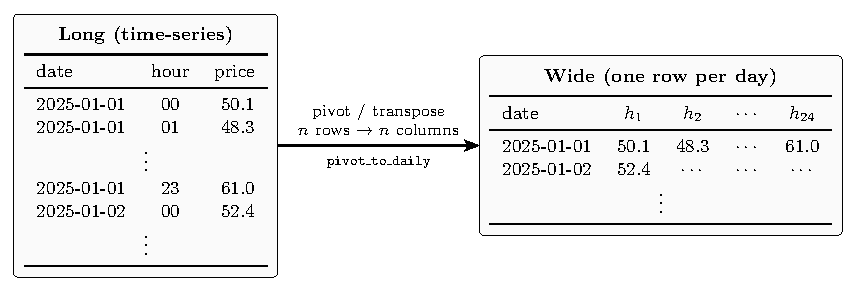
\includegraphics[width=\linewidth]{f-pivot-wide}
    \end{column}
  \end{columns}
\end{frame}

\begin{frame}{Backup --- the two deep architectures \hfill\small(\S3.3.2--3.3.3)}
  \begin{columns}[c]
    \begin{column}{0.5\textwidth}
      \centering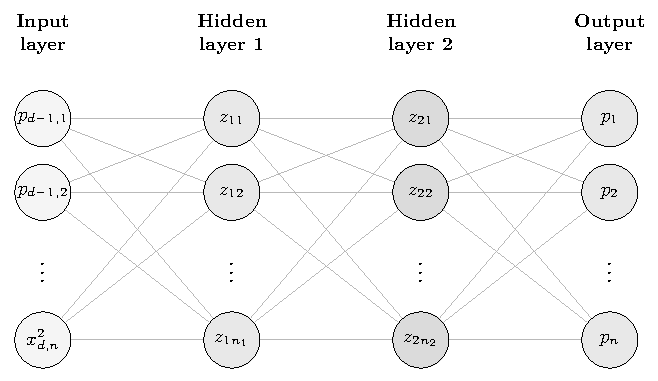
\includegraphics[height=4.4cm]{f-dnn-architecture}\\{\scriptsize DNN (MIMO MLP)}
    \end{column}
    \begin{column}{0.5\textwidth}
      \centering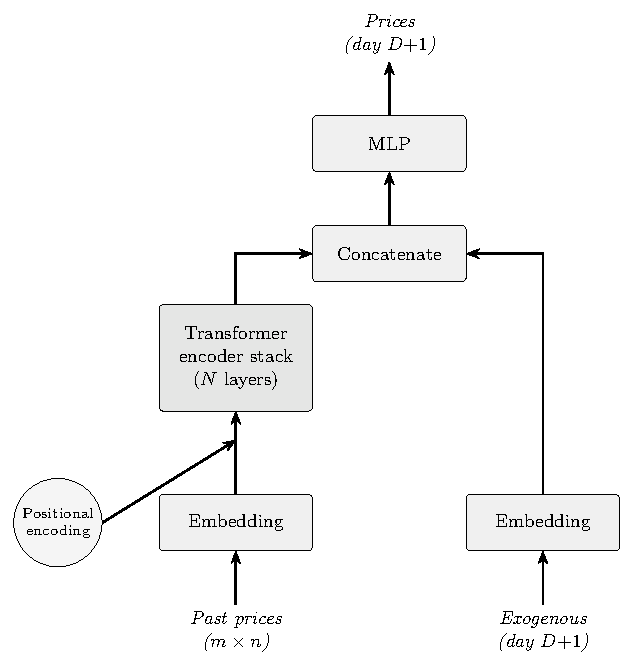
\includegraphics[height=4.4cm]{f-transformer-flow}\\{\scriptsize Transformer}
    \end{column}
  \end{columns}
\end{frame}

\begin{frame}{Backup --- recalibration, evaluation, tuning \hfill\small(\S3.4--3.7)}
  \begin{columns}[c]
    \begin{column}{0.5\textwidth}
      \centering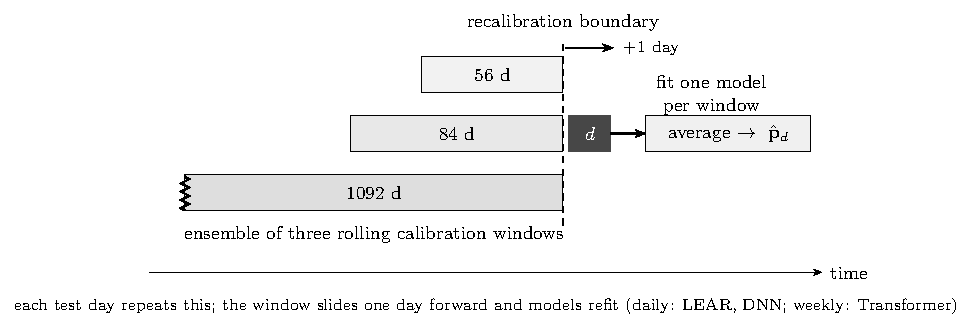
\includegraphics[width=\linewidth]{f-recalibration}
    \end{column}
    \begin{column}{0.5\textwidth}
      \begin{itemize}\small
        \item Rolling walk-forward; forecasts averaged over a calibration-window ensemble;
          daily refit (LEAR, DNN), weekly (Transformer).
        \item Metrics MAE / RMSE / sMAPE / rMAE; paired GW tests.
        \item DNN tuned by Optuna TPE (6 HPs) on an ex-ante validation window.
      \end{itemize}
    \end{column}
  \end{columns}
\end{frame}

\begin{frame}{Backup --- why the Transformer is third}
  \begin{columns}[c]
    \begin{column}{0.5\textwidth}
      \centering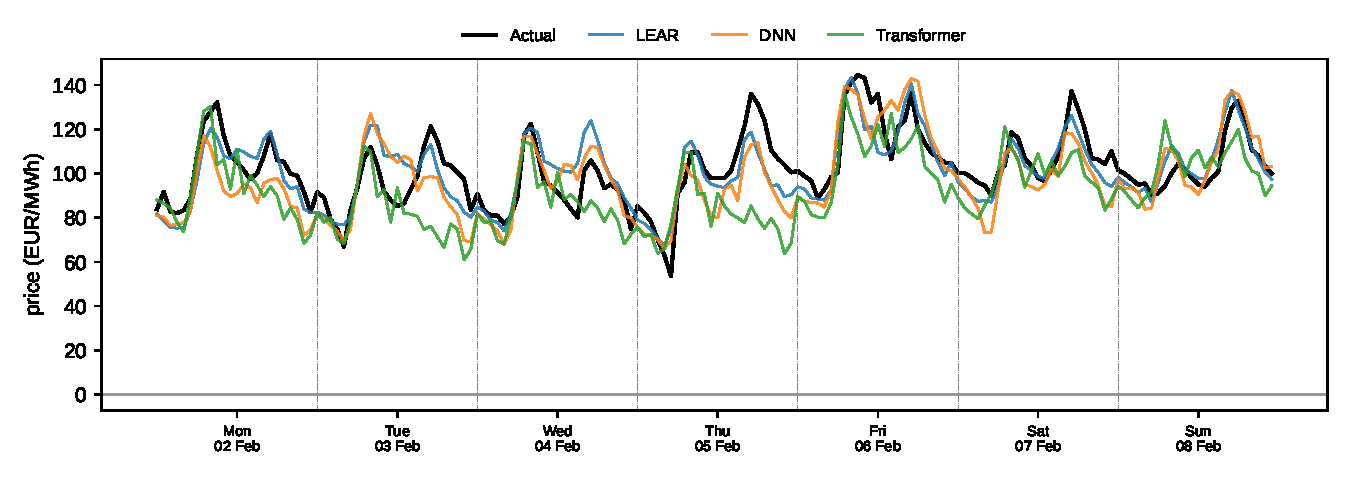
\includegraphics[width=\linewidth]{forecast_calm_dk1}\\{\scriptsize Calm week}
    \end{column}
    \begin{column}{0.5\textwidth}
      \centering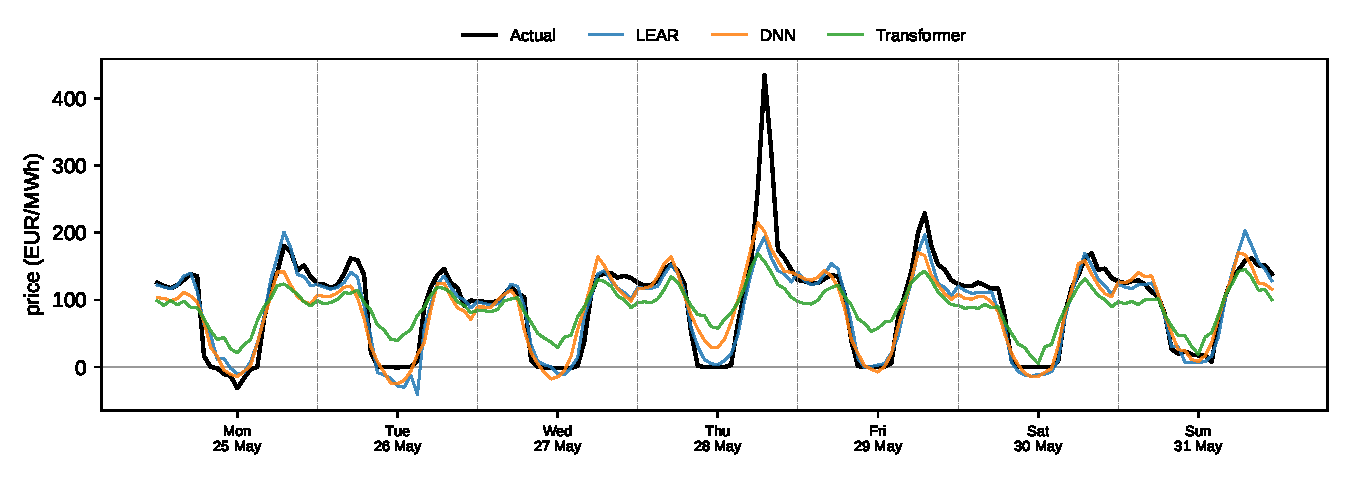
\includegraphics[width=\linewidth]{forecast_renew_dk1}\\{\scriptsize Renewable week}
    \end{column}
  \end{columns}
  \vskip0.3em
  \centering\footnotesize It smooths over the negative hours and the scarcity peak; LEAR and
  the DNN follow them.
\end{frame}

\begin{frame}{Backup --- Giacomini--White vs Diebold--Mariano}
  GW regresses the daily loss differential on an instrument set:
  \[ \Delta^{A,B}_d = \phi' X_{d-1} + \varepsilon_d . \]
  \begin{itemize}\footnotesize
    \item $X_{d-1}$ = constant \emph{and} lagged differentials $\to$ conditional predictive
      ability.
    \item $X_{d-1}$ = \textbf{constant only} (Lago eq.~15) $\to$ multivariate \textbf{DM},
      which is what I compute, with Newey--West HAC errors (lag $\lfloor T^{1/4}\rfloor$).
      I follow Lago's naming; I do not exercise the conditioning.
  \end{itemize}
\end{frame}

\begin{frame}{Backup --- "Tied" means indistinguishable, not equal}
  \begin{itemize}
    \item $p=0.16$ is a \textbf{non-rejection}, not proof of equality.
    \item $n\approx187$ daily differentials; the gap is $\sim$3\% relative --- power is low.
    \item Equality would need a TOST / equivalence test; I claim \textbf{indistinguishability}.
    \item No multiplicity correction, but the load-bearing results clear any correction by
      orders of magnitude.
  \end{itemize}
\end{frame}

\begin{frame}{Backup --- documented deviations from the papers \hfill\small(Table 3.4)}
  \footnotesize
  \begin{tabular}{lll}
    \toprule
    Aspect & Paper & This work (reason) \\
    \midrule
    Test length      & $\ge$1--2 years        & 31 weeks (data history) \\
    DNN tuning        & 1500 TPE iters         & 30 trials (compute) \\
    DNN search space  & arch + feature selectors & architecture only \\
    LEAR windows      & 56/84/1092/1456 d      & 56/84/1092 d (1456 predates data) \\
    DNN window        & 4 years                & 730 d \\
    $\lambda$ select  & LARS+AIC               & \texttt{LassoCV} (close, standard) \\
    Resolution        & hourly                 & 15-min $\to$ hourly mean \\
    Transformer regime& train-once + renorm    & rolling window + weekly refit \\
    Transformer HPs   & tuned per dataset      & paper defaults reused \\
    \bottomrule
  \end{tabular}
\end{frame}

\end{document}
